\chapter{Background}\label{chapter:background}

In this Chapter are analyzed theoretical aspects behind Reservoir Computing (RC), with a focus on Echo State Networks (ESNs). Next, we will address Federated Learning (FL) along with two different FL algorithms: \texttt{FedAvg} and \texttt{FedCurv}. Finally, we will discuss the specific aspect of FL applied to ESNs.

\section{Reservoir Computing and Echo State Networks}

Artificial Recurrent Neural Networks (RNNs) represent a large and varied class of computational models that are designed in analogy with biological brain modules. In an RNN numerous abstract neurons (also called units or processing elements) are interconnected by likewise abstracted synaptic connections (or links), which enable activations to propagate through the network. The characteristic feature of RNNs that distinguishes them from the feedforward neural networks is that the connection topology possesses feedback loops. Such loops enable the RNNs to may develop a self-sustained temporal activation dynamics along its recurrent connection pathways, even in the absence of input. Mathematically, RNNs enrich feedforward neural networks by introducing the temporal component in the equation, making it a dynamical system modelled by its corresponding differential equation. If driven by an input signal, an RNN preserves in its internal state a nonlinear transformation of the input history, in other words, it has a dynamical memory, and is able to process temporal context information \cite{lukovsevivcius2009reservoir}. \\

The main shortcoming of RNNs is that they are difficult to train by gradient-descent-based methods, which aim at iteratively reducing the training error. The reasons behind such difficulty are twofold. First, gradual change of network parameters during learning drives the network dynamics through bifurcations \cite{doya1992bifurcations}. At such points, the gradient information degenerates and may become ill-defined. As a consequence, convergence cannot be guaranteed. Second, computing the gradient of the error requires unfolding the network over time, which increases the computational cost of the learning algorithm and may make it unfeasible depending on the size of the model and the supporting hardware. Another shortcoming is represented by the difficulty of learning long-term dependencies, since the necessary gradient information exponentially dissolves over time \cite{bengio1994learning}. Long Short-Term Memory (LSTM) networks represents a possible solution \cite{gers2000learning}. However, besides the difficulty of handling its corresponding learning algorithms \cite{lukovsevivcius2009reservoir}, this model still falls back in the shortcoming described above. \\

In this situation of slow and difficult progress, in 2001 a fundamentally new approach to RNN design and training was proposed by Wolfgang Maass under the name of Liquid State Machines \cite{maass2002real} and by Herbert Jaeger under the name of Echo State Networks (ESNs) \cite{jaeger2001echo}. This approach is often referred to as Reservoir Computing (RC). The RC paradigm avoids the shortcomings of gradient-descent RNN training stated above, by setting up RNNs in the following way:

\begin{itemize}
    \item A Recurrent Neural Network is \textit{randomly} created and remains unchanged during training. This RNN is called the \textit{reservoir}. It is passively excited by the input signal and maintains in its state a nonlinear transformation of the input history.
    
    \item The desired output signal is generated as a linear combination of the neuron’s signals from the input-excited reservoir. This linear combination, named \textit{readout}, is obtained by linear regression, using the teacher signal as a target.
\end{itemize}

\subsection{Echo State Network Formalization}

Let a \textit{problem} or a \textit{task} in our context of machine learning be defined as a problem of learning a functional relation between a given input $\textbf{u}(t) \in \mathbb{R}^{N_u}$ and a desired output $\textbf{y}_{target}(t) \in \mathbb{R}^{N_y}$, where $t=1,\dots ,T$, and $T$ is the number of data points in the training \textit{dataset} $\{(\textbf{u}(t), \textbf{y}_{target}(t))\}$. In a \textit{temporal task} the function to be learned depends on the history of the input, so the expansion function has memory: $\textbf{x}(t)=x(\dots, \textbf{u}(t-1), \textbf{u}(t))$, i.e., it is an expansion of the current input and its (potentially infinite) history. Since this function has an unbounded number of parameters, practical implementations often take an alternative, recursive, definition:

\begin{equation}\label{eq:temporal_task}
    \textbf{x}(t)=x(\textbf{x}(t-1), \textbf{u}(t)).
\end{equation}

The type of Recurrent Neural Networks that we will consider in this Work is a straightforward implementation of Eq. \ref{eq:temporal_task} where a nonlinear expansion with memory here leads to a \textit{state vector} of the form:

\begin{equation}\label{eq:reservoir_state}
    \textbf{x}(t)=f(\textbf{W}_{in}\textbf{u}(t)+\widehat{\textbf{W}}\textbf{x}(t-1)), t=1,\dots , T.
\end{equation}

where $\textbf{x}(t) \in \mathbb{R}^{N_x}$ is a vector of reservoir neuron activations at a time step $t$, $f(\cdot)$ is the neuron activation function, usually the $tanh(\cdot)$, $\textbf{W}_{in} \in \mathbb{R}^{N_x \times N_u}$ is the input weight matrix, and $\widehat{\textbf{W}} \in \mathbb{R}^{N_x \times N_x}$ is a weight matrix of internal network connections. The network is usually started with the initial state $\textbf{x}(0)=0$.
The \textit{readout} of the network is implemented in this way:

\begin{equation}\label{eq:readout}
    \textbf{y}(t)=f_{out}(\textbf{W}\textbf{x}(\textbf{u}(t)))
\end{equation}

where $f_{out}(\cdot)$ is a nonlinear function (e.g., a sigmoid applied element-wise), $\textbf{W} \in \mathbb{R}^{N_y \times N_x}$ are the trained output weights. \\

Echo State Networks \cite{jaeger2007echo} represent one of the two pioneering reservoir computing methods. The approach is based on the observation that if a random RNN possesses certain algebraic properties, training only a linear readout from it is often sufficient to achieve excellent performance in practical applications. The untrained layer of the ESN is called a \textit{dynamic reservoir}, and the resulting states $\textbf{x}(t)$ are termed \textit{echoes} of its input history \cite{jaeger2001echo}, this is where Reservoir Computing draws its name from. \\

\begin{center}
\begin{minipage}[c]{\textwidth}
    \centering
    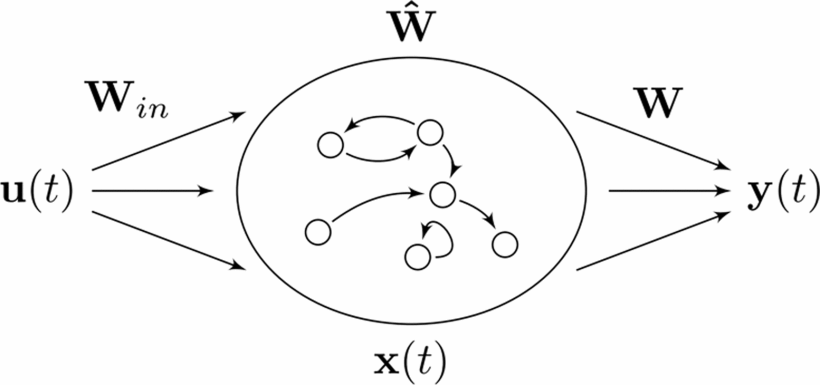
\includegraphics[width=0.6\textwidth]{contents/Chapter2/esn-arch.png}
    \captionof{figure}{Architecture of an ESN. The input signal $\textbf{u}(t)$ is fed to the recurrent reservoir. Then, a state $\textbf{x}(t)$ is extracted from the reservoir, from which an output $\textbf{y}(t)$ is computed \cite{bacciu2021federated}}
    \label{fig:esn_arch}
\end{minipage}
\end{center}

A fundamental constraint of the ESNs is that we must ensure the stability of the dynamical system. Such constraint is satisfied by the \textit{Echo State Property} (ESP) \cite{jaeger2001echo} (Def. \ref{def:esp}). Apply the sufficient condition (Theorem \ref{thm:suff_cond_esp}) for the ESP is fine in theory, but often impractical because it is too strong. Usually, the necessary condition (Theorem \ref{thm:nec_cond_esp}) is used as an easy way for initialization of the reservoir. \\

The necessary condition states that the effect of a previous state $\textbf{x}(t)$ and a previous input $\textbf{u}(t)$ on a future state $\textbf{u}(t+k)$ should vanish gradually as time passes (i.e. $k\rightarrow\infty$), and not persist or even get amplified \cite{lukovsevivcius2009reservoir}. For most practical purposes, the ESP is assured if the reservoir weight matrix $\widehat{\textbf{W}}$ is scaled so that its spectral radius $\rho(\widehat{\textbf{W}})$ (i.e., the largest absolute eigenvalue) satisfies $\rho(\widehat{\textbf{W}})<1$ \cite{jaeger2001echo} or, using
another term, $\widehat{\textbf{W}}$ is \textit{contractive}. Practically, the initialization of $\widehat{W}$ is made in the following way:

\begin{equation}
    \widehat{\textbf{W}} \leftarrow \widehat{\textbf{W}} \frac{\rho_{desired}}{\rho(\widehat{\textbf{W}})}
\end{equation}

where $\rho_{desired} < 1$. Also the $\textbf{W}_{in}$ matrix could be initialized in the following way:

\begin{equation}
    \textbf{W}_{in} \leftarrow \omega_{in}\textbf{W}_{in}
\end{equation}

where $\omega_{in}$ is the \textit{input scaling} parameter that makes $\textbf{W}_{in}$ values falling in the interval $[-\omega_{in}, \omega_{in}]$ if the elements of $\textbf{W}_{in}$ are generated randomly from a uniform distribution on the interval $[-1,1]$. The spectral radius $\rho(\widehat{\textbf{W}})$ and the input scaling $\omega_{in}$ are key hyper-parameters of the reservoir initialization. \\


\begin{definition}[Reservoir State Transition Function]\label{def:rstf}
Given $N_u$ the input dimension and $N_x$ the number of reservoir neurons. The reservoir is a discrete-time input-driven dynamical system, and its dynamics are driven by the State Transition Function:

\begin{equation}\nonumber
    F:\mathbb{R}^{N_u} \times \mathbb{R}^{N_x} \rightarrow \mathbb{R}^{N_x}
\end{equation}

\begin{equation}
    \textbf{x}(t)=F(\textbf{u}(t), \textbf{x}(t-1))
\end{equation}

where $F$ takes an input and a state and returns a new state. The final state after seeing an entire input sequence s, given the initial state, is given by the iterative version of the State Transition Function:

\begin{equation}\nonumber
    \widehat{F}:(\mathbb{R}^{N_u})^* \times \mathbb{R}^{N_x} \rightarrow \mathbb{R}^{N_x}
\end{equation}

\begin{equation}
    \widehat{F}(s,x_0)=\left\{\begin{matrix}x_0 & \textup{if s=[ ]}\\F(x(t), \widehat{F}([x(1),\dots, x(t-1)],x_0)) & \textup{if s=[x(1),\dots, x(t)]}
\end{matrix}\right.
\end{equation} \\
\end{definition}


\begin{definition}[Echo State Property (ESP)]\label{def:esp}
Given $N_u$ the input dimension, $N_x$ the number of reservoir neurons and the State Transition Function $\widehat{F}$ (Def. \ref{def:rstf}). An ESN satisfies the ESP whenever:

\begin{equation}\nonumber
    \forall s \in (\mathbb{R}^{N_u})^N, \forall x_0,z_0 \in \mathbb{R}^{N_x}:
\end{equation}

\begin{equation}
    \left\| \widehat{F}(s, x_0)-\widehat{F}(s, z_0) \right\| \rightarrow 0, \text{\quad as\quad} N \rightarrow \infty
\end{equation}

briefly, given the input sequence and two initial states, the distance between the final stages goes to 0 with the length of the input. \\
\end{definition}


\begin{theorem}[Sufficient Condition for the ESP]\label{thm:suff_cond_esp}
If the maximum singular value of $\widehat{W}$ is less than 1 the ESN satisfies the ESP for any possible input.

\begin{equation}
    \sigma_{max}(\widehat{W})=\left\| \widehat{W} \right\|_2 < 1
\end{equation}

in other therms, there is a contractive dynamics for every input. \\
\end{theorem}


\begin{theorem}[Necessary Condition for the ESP]\label{thm:nec_cond_esp}
If the spectral radius of $\widehat{W}$ is not smaller than 1 the ESN does not satisfies the ESP.

\begin{equation}
    \rho(\widehat{W})=\max(abs(eig(\widehat{W})) < 1
\end{equation}

in other therms, there is a globally asymptotically stable dynamics around the 0 state. \\
\end{theorem}


ESNs (Def. \ref{def:esn}) standardly computes the reservoir states as in Eq. \ref{eq:reservoir_state}, where the nonlinear function $f(\cdot)$ is a sigmoid, usually the $tanh(\cdot)$ function. Leaky integrator neuron models represent another frequent option for ESNs (Def. \ref{def:liesn}), and is the one used in this Work and named Li-ESNs. \\

\begin{definition}[ESN]\label{def:esn}
Given $N_u$ the input dimension, $N_x$ the number of reservoir neurons, $N_y$ the output dimension and $\textbf{x}(0)=0$, the ESN at each time step $t \in \{1,\dots, T\}$ computes the state vector $\textbf{x}(t) \in \mathbb{R}^{N_x}$ for a given input signal $\textbf{u}(t) \in \mathbb{R}^{N_u}$ as:

\begin{equation}\nonumber
    \textbf{x}(t)=\tanh(\textbf{W}_{in}\textbf{u}(t)+\widehat{\textbf{W}}\textbf{x}(t-1)).
\end{equation}

where $\textbf{W}_{in} \in \mathbb{R}^{N_x \times N_u}$ and $\widehat{\textbf{W}} \in \mathbb{R}^{N_x \times N_x}$ are fixed and untrained. The readout of the network $\textbf{y}(t) \in \mathbb{R}^{N_y}$ is computed as:

\begin{equation}\nonumber
    \textbf{y}(t)=sigmoid(\textbf{W}x(\textbf{u}(t)))
\end{equation}

where $\textbf{W} \in \mathbb{R}^{N_y \times N_x}$ is trainable. \\\\
\end{definition}



\begin{definition}[Li-ESN]\label{def:liesn}
Given $N_u$ the input dimension, $N_x$ the number of reservoir neurons, $N_y$ the output dimension, $\textbf{x}(0)=0$ and $\alpha \in \mathbb{R}$ the leaking rate $(0<\alpha\leq1)$, the Li-ESN at each time step $t \in \{1,\dots, T\}$ computes the state vector $\textbf{x}(t) \in \mathbb{R}^{N_x}$ for a given input signal $\textbf{u}(t) \in \mathbb{R}^{N_u}$ as:

\begin{equation}\nonumber
    \textbf{x}(t)=(1-\alpha)\textbf{x}(t-1)+\alpha \tanh(\textbf{W}_{in}\textbf{u}(t)+\widehat{\textbf{W}}\textbf{x}(t-1)).
\end{equation}

where $\textbf{W}_{in} \in \mathbb{R}^{N_x \times N_u}$ and $\widehat{\textbf{W}} \in \mathbb{R}^{N_x \times N_x}$are fixed and untrained. The readout of the network $\textbf{y}(t) \in \mathbb{R}^{N_y}$ is computed as:

\begin{equation}\nonumber
    \textbf{y}(t)=sigmoid(\textbf{W}x(\textbf{u}(t)))
\end{equation}

where $\textbf{W} \in \mathbb{R}^{N_y \times N_x}$ is trainable.
\end{definition}


\section{Federated Learning}

Nowadays phones and tablets are the primary computing devices for many people \cite{poushter2016smartphone}\cite{anderson2015technology}. The powerful sensors on these devices (including cameras, microphones, and GPS), combined with the fact they are frequently carried, means they have access to an unprecedented amount of data, much of it private in nature. Models learned on such data hold the promise of greatly improving usability by powering more intelligent applications, but the sensitive nature of the data means there are risks and responsibilities to storing it in a centralized location. \\

Recently, the concept of Federated Learning (FL) has been proposed for building intelligent and privacy-enhanced IoT systems. Technically, FL is a distributed collaborative AI approach that allows for data training by coordinating multiple devices with a central server without sharing actual datasets \cite{konevcny2016federated}. \\

For instance, multiple IoT devices can act as workers to communicate with an aggregator (e.g. a server) for performing neural network training in intelligent IoT networks. More specifically, the aggregator first initiates a global model with
learning parameters. Each worker downloads the current model from the aggregator, computes its model update (e.g. Stochastic Gradient Descent) by using its local dataset, and sends the computed local update back to the aggregator. \\

Then, the aggregator combines all local model updates and constructs a new improved global model. By using the computing power of distributed workers, the aggregator can enhance the training quality while minimizing user privacy leakage. \\

Finally, the local workers download the global update from the aggregator, and compute their next local update until the global training is complete \cite{nguyen2021federated}.


\subsection{Federated Averaging}

Google researchers, in 2017, proposed \textit{FederatedAveraging} (or \texttt{FedAvg}) \cite{mcmahan2017communication} algorithm that makes as contributions 1) the identification of the problem of training on decentralized data from mobile devices while complying to privacy constraints as an important research direction; 2) the selection of a straightforward and practical algorithm that can be applied to this setting; and 3) an extensive empirical evaluation of the proposed approach. \texttt{FedAvg} is a general implementation of \texttt{FedSGD} and more concretely, it combines local stochastic gradient descent (SGD) on each client with a server that performs model averaging. It is robust to unbalanced and non-IID data distributions, and can reduce the rounds of communication needed to train a deep network on decentralized data by orders of magnitude. \\

It addresses the key issues of client availability and unbalanced and non-IID data. It assumes also a synchronous update scheme that proceeds in rounds of communication. There is a fixed set of $K$ clients, each with a fixed local dataset. At the beginning of each round, a random fraction $C$ of clients is selected, and the server sends the current global algorithm state to each of these clients (e.g., the current model parameters). Each selected client then performs local computation based on the global state and its local dataset, and sends an update to the server. The server then applies these updates to its global state, and the process repeats. \\

\begin{figure}[H]\label{fig:fedavg}
\centering
\begin{tikzpicture}[scale=2]
  \draw[line width=0pt]
    (2,2) node[draw] (s) {server}
    (0,0)  node[draw] (c1) {client $c_1$}
    (4,0)  node[draw] (cn) {client $c_n$}
    (2,0)  node[draw=none] (d) {$\dots$};

  \draw[->] (2,1)--(c1.north east);
  \draw[->] (2,1)--(cn.north west);
  \draw (2,1)-- node[right] {\textbf{W}} (s);
  \draw[->] (c1.north)-- node[left] {$\textbf{W}_{c_1}$} (0,2)--(s.west);
  \draw[->] (cn.north)-- node[right] {$\textbf{W}_{c_n}$} (4,2)--(s.east);
\end{tikzpicture}
\caption{Federated Averaging Scheme. Each client $c$ sends their local matrix $\textbf{W}_c$ to the server. After the aggregation of the models is performed in the form of a weighted average, the server sends back the same matrix $\textbf{W}$ to all clients \cite{bacciu2021federated}.}
\end{figure}

The algorithm considered is applicable to any finite-sum objective of the form:

\begin{equation}\label{eq:fedavg_obj}
    \min_{w\in\mathbb{R}^d}f(w) \textup{\quad where\quad} f(w)=\frac{1}{n}\sum_{i=1}^{n}f_i(w).
\end{equation}

For a machine learning problem, we typically take $f_i(w)=\ell(x_i,y_i;w)$, that is, the loss of the prediction on example $(x_i,y_i)$ made with model parameters $w$. We assume there are $K$ clients over which the data is partitioned, with $\mathcal{P}_k$ the set of indexes of data points on client $k$, with $n_k=\left| \mathcal{P}_k \right|$. Thus, we can rewrite the objective in Eq. \ref{eq:fedavg_obj} as:

\begin{equation}
    f(w)=\sum_{i=1}^{K}\frac{n_k}{n}F_k(w) \text{\quad where\quad} F_k(w)=\frac{1}{n_k}\sum_{i\in\mathcal{P}_k}f_i(w).
\end{equation}

If the partition $\mathcal{P}_k$ was formed by distributing the training examples over the clients uniformly at random, then we would have $\mathbb{E}_{\mathcal{P}_k}\left[ F_k(w) \right]=f(w)$, where the expectation is over the set of examples assigned to a fixed client $k$. This is the IID assumption typically made by distributed optimization algorithms; \texttt{FedAvg} refers to the case where this does not hold (that is, $F_k$ could be an arbitrarily bad approximation to $f$) as the non-IID setting. \\

The multitude of successful applications of deep learning have almost exclusively relied on variants of SGD for optimization, and can be applied naively to the federated optimization problem. This is done selecting a $C$-fraction of clients on each round, and compute the gradient of the loss over all the data held by these clients. Thus, $C$ controls the \textit{global} batch size, with $C=1$ corresponding to full-batch (non-stochastic) gradient descent. This is the baseline algorithm named \textit{FederatedSGD} (or \texttt{FedSGD}). \\

A typical implementation of \texttt{FedSGD} with $C=1$ and a fixed learning rate $\eta$ has each client $k$ compute $g_k=\nabla F_k(w_t)$, the average gradient on its local data at the current model $w_t$, and the central server aggregates these gradients and applies the update $w_{t+1}\leftarrow w_t-\eta \sum_{k=1}^{K}\frac{n_k}{n}g_k$, since $\sum_{k=1}^{K}\frac{n_k}{n}g_k=\nabla f(w_t)$. An equivalent update is given by $\forall k, w_{t+1}^k\leftarrow w_t-\eta g_k$ and then $w_{t+1}\leftarrow \sum_{k=1}^K\frac{n_k}{n}w_{t+1}^k$. That is, each client locally takes one step of gradient descent on the current model using its local data, and the server then takes a weighted average of the resulting models. \\

Once the algorithm is written this way, we can add more computation to each client by iterating the local update $w^k\leftarrow w^k-\eta F_k(w^k)$ multiple times before the averaging step. This approach is named \textit{FederatedAveraging} (or \texttt{FedAvg}). The amount of computation is controlled by three key parameters: $C$, the fraction of clients that perform computation on each round; $E$, then number of
training passes each client makes over its local dataset on each round; and $B$, the local minibatch size used for the client updates. With $B=\infty$ it means that the full local dataset is treated as a single minibatch. Thus, at one endpoint of this algorithm family, we can take $B=\infty$ and $E=1$ which corresponds exactly to \texttt{FedSGD}. For a client with $n_k$ local examples, the number of local updates per round is given by $u_k=E\frac{n_k}{B}$. The pseudo-code is given in Alg. \ref{alg:fedavg}.


\algrenewcommand\algorithmicfunction{}
\algrenewcommand\textproc{}
\begin{algorithm}[H]
\caption{\texttt{FedAvg}. The $K$ clients are indexed by $k$; $B$ is the local minibatch size, $E$ is the number of local epochs, and $\eta$ is the learning rate.}\label{alg:fedavg}
\begin{algorithmic}[1]
\Function{\textbf{ServerUpdate}}{}
    \State $w_0\leftarrow$ initialize()
    \For{\texttt{each round $t=1,2,\dots$}}
        \State $m\leftarrow \max(C\cdot K, 1)$
        \State $S_t\leftarrow \text{(random set of $m$ clients)}$
        \For{\texttt{each client $k\in S_t$}}
            \State $w_{t+1}^k\leftarrow$ \text{ClientUpdate($k$, $w_t$)}
        \EndFor
        \State $w_{t+1}\leftarrow \sum_{k=1}^K\frac{n_k}{n}w_{t+1}^k$
    \EndFor
\EndFunction
\\
\Function{\textbf{ClientUpdate}}{$k$, $w$}
    \State $\mathcal{B}\leftarrow \text{(split $\mathcal{P}_k$ into batches of size $B$)}$
    \For{\texttt{$i$ from $1$ to $E$}}
        \For{\text{batch $b\in \mathcal{B}$}}
            \State $w\leftarrow w-\eta\nabla\ell(w;b)$
        \EndFor
    \EndFor
    \Return $w$
\EndFunction
\end{algorithmic}
\end{algorithm}


\subsection{Federated Curvature}\label{sec:fedcurv}

Federated Learning on non-IID distributions has trouble achieving good results in terms of accuracy and the number of communication rounds \cite{mcmahan2017communication}. There is a deep parallel between the FL problem and another fundamental machine learning problem called \textit{Lifelong Learning}. In Lifelong Learning, the challenge is to learn task A, and continue on to learn task B using the same model, but without "forgetting", without severely hurting the performance on task A. In general, it is a problem of learning tasks $A_1, A_2, \dots$ in sequence without forgetting previously-learnt tasks for which samples are not presented anymore. In the Federated Learning context, the previous problem is translated in how to learn a task without disturbing different ones learnt on the same model. An approach to this kind of problem that preserves privacy and communication offload, may be found in \textit{Elastic Weight Consolidation} (EWC) \cite{kirkpatrick2017overcoming}. \\

EWC aims to prevent catastrophic forgetting when moving from learning task A to learning task B. The idea is to identify the coordinates in the network parameters $\theta$ that are the most informative for task $A$, and then, while task $B$ is being learned, penalize the learner for changing these parameters. The basic assumption is that deep neural networks are over-parameterized enough, so that there are good chances of finding an optimal solution $\theta_B^*$ to task $B$ in the neighborhood of previously learned $\theta_A^*$. In order to control the stiffness of $\theta$ per coordinate while learning task $B$, EWC uses the diagonal of the Fisher information matrix $\mathcal{I}_A^*=\mathcal{I}_A(\theta_A^*)$ to selectively penalize parts of the parameters vector $\theta$ that are getting too far from $\theta_A^*$ \cite{kirkpatrick2017overcoming}. This is done using the following objective:

\begin{equation}\label{eq:ewc_obj}
    \Tilde{L}(\theta)=L_B(\theta)+\lambda(\theta-\theta_A^*)^T diag(\mathcal{I}_A^*)(\theta-\theta_A^*)
\end{equation}

The formal justification provided for Eq. \ref{eq:ewc_obj} is Bayesian: Let $D_A$ and $D_B$ be independent datasets used for tasks $A$ and $B$. We have that:

\begin{equation}
    \log p(\theta|D_A,D_B)=\log p(D_B|\theta)+\log p(\theta|D_A)-\log p(D_B)
\end{equation}

where $\log p(D_B|\theta)$ is just the standard likelihood maximized in the optimization of $L_B(\theta)$, and the posterior $\log p(\theta|D_A)$ is approximated with Laplace’s method as a Gaussian distribution with expectation $\theta_A^*$ and covariance $diag(\mathcal{I}_A^*)$. \\ 

It is also well known that under some regularity conditions, the information matrix approximates the Hessian $H_L$ of $L(\theta)$, at $\theta=\theta^*$ \cite{pronzato2013design}. By this we get a non Bayesian interpretation of Eq. \ref{eq:ewc_obj}:

\begin{equation}
    \Tilde{L}(\theta)\approx L_B(\theta)+\frac{1}{2}(\theta-\theta_A^*)^T H_{L_A}(\theta-\theta_A^*)\approx L_B(\theta)+L_A(\theta)
\end{equation}

where $L(\theta)=L_B(\theta)+L_A(\theta)$ is exactly the loss we want to minimize. \\

\textit{Federated Curvature} (or \texttt{FedCurv}) is an adaptation of the EWC algorithm to the Federated Learning scenario. We mark by $S=\{1, \dots, N\}$ the $N$ nodes as a task with local datasets $\{A_1, \dots, A_N\}$. At this step we consider each nodes in $S$, instead a subset of them as in \texttt{FedAvg} (but can be extended to select a subset). At round $t$ each node $s\in S$ optimizes the following loss:

\begin{equation}\label{eq:fedcurv_obj}
    \Tilde{L}_{t,s}=L_s(\theta)+\lambda\sum_{j\in S\backslash s}(\theta-\Tilde{\theta}_{t-1,j})^T diag(\Tilde{\mathcal{I}}_{t-1,j})(\theta-\Tilde{\theta}_{t-1,j}).
\end{equation}

On each round $t$, starting from initial point $\Tilde{\theta}_t=\frac{1}{N}\sum_{i=1}^N \Tilde{\theta}_{t-1,i}$, the nodes optimize their local loss by running SGD for $E$ local epochs. At the end of each round $t$, each node $j$ sends to the rest of the nodes the SGD result $\Tilde{\theta}_{t,j}$ and $diag(\Tilde{\mathcal{I}}_{t,j})$ that will be used for the loss of round $t+1$. \\

\texttt{FedCurv} might look cumbersome and expensive to store and transmit. However by careful implementation we can avoid it, so Eq. \ref{eq:fedcurv_obj} can be arranged as in Eq. \ref{eq:fedcurv_obj_rev}

\begin{equation}\label{eq:fedcurv_obj_rev}
    \Tilde{L}_{t,s}=L_s(\theta)+\lambda\theta^T\left[ \sum_{j\in S\backslash s} diag(\Tilde{\mathcal{I}}_{t-1,j}) \right]\theta-2\lambda\theta^T \sum_{j\in S\backslash s} diag(\Tilde{\mathcal{I}}_{t-1,j})\Tilde{\theta}_{t-1,j}+\text{const}
\end{equation}

The central point needs only two additional elements to maintain and transmit, of the same size of $\theta$, and are $u_t$ and $v_t$, as shown in Eq. \ref{eq:u_and_v}

\begin{equation}\label{eq:u_and_v}
    u_t=\sum_{j\in S} diag(\Tilde{\mathcal{I}}_{t-1,j}) \text{\quad and \quad} v_t=\sum_{j\in S} diag(\Tilde{\mathcal{I}}_{t-1,j})\Tilde{\theta}_{t-1,j}
\end{equation}

The device can then construct the data needed for the evaluation of $\Tilde{L}$ from $u_t$ and $v_t$ by subtraction. \\

The specific implementation of the algorithm, is presented in Chapter \ref{chapter:fedcurv}.


\section{Federated Echo State Networks}

There is a vast amount of literature regarding federated RNNs, but here we focus on the paradigm of Reservoir Computing, which allows to produce highly resource-efficient RNNs \cite{bacciu2021federated}. Specifically, it is used the Li-ESN as described in the Def. \ref{def:liesn} in a FL setting. In this context we consider only the trainable weight matrix $\textbf{W}$ and the training proceeds as follows:

\begin{enumerate}
    \item the input sequences from the training dataset are fed to the reservoir
    \item the relevant states on which the network must learn to perform predictions are collected column-wise into a matrix $\textbf{S}\in \mathbb{R}^{N_x\times N_{train}}$, where $N_{train}$ is the number of such states, and the associated targets are collected into the matrix $\textbf{Y}\in \mathbb{R}^{N_y\times N_{train}}$
    \item the matrix $\textbf{W}$ is obtained as the solution to a least squares minimization problem between $\textbf{WS}$ and $\textbf{Y}$.
\end{enumerate}

In particular, a common algorithm for a regularized solution to the least squares problem is ridge regression. In this case, if $\beta\in \mathbb{R}^+$ is the L2 regularization factor chosen by model selection, the readout weights are computed in closed form as follows:

\begin{equation}\label{eq:pseudo_inv}
    \textbf{W}=\textbf{Y}\textbf{S}^T(\textbf{S}\textbf{S}^T+\beta\textbf{I})^{-1}
\end{equation}

The method proposed as \textit{Incremental Federated Learning} (or \texttt{IncFed}) \cite{bacciu2021federated}, uses peculiar characteristics of ESN training allowing an optimal form of federated learning. Locally, instead of computing the readout weights, each client \textit{c} computes the matrices $\textbf{A}_c\in \mathbb{R}^{N_y\times N_x}$ and $\textbf{B}_c\in \mathbb{R}^{N_x\times N_x}$ as follow:

\begin{equation}
    \textbf{A}_c=\textbf{Y}_c\textbf{S}_c^T\text{\quad and\quad}\textbf{B}_c=\textbf{S}_c\textbf{S}_c^T+\beta_c\textbf{I}
\end{equation}

The matrices $\textbf{A}_c$ and $\textbf{B}_c$ are sent to the server where they get summed as in the following equations:

\begin{equation}
    \textbf{A}=\sum_{c\in\mathcal{C}}\textbf{A}_c\text{\quad and\quad}\textbf{B}=\sum_{c\in\mathcal{C}}\textbf{B}_c
\end{equation}

After the summed matrices are computed, the server can compute the optimal readout weights $\textbf{W}$ in closed-form as follows:

\begin{equation}\label{eq:pseudo_inv_fed}
    \textbf{W}=\textbf{A}\textbf{B}^{-1}
\end{equation}

Notice how Eq. \ref{eq:pseudo_inv_fed} is mathematically equivalent to Eq. \ref{eq:pseudo_inv} if all data was locally available to the server. \\



\begin{figure}[H]\label{fig:incfed}
\centering
\begin{tikzpicture}[scale=2]
  \draw[line width=0pt]
    (2,2) node[draw] (s) {server}
    (0,0)  node[draw] (c1) {client $c_1$}
    (4,0)  node[draw] (cn) {client $c_n$}
    (2,0)  node[draw=none] (d) {$\dots$};

  \draw[->] (2,1)--(c1.north east);
  \draw[->] (2,1)--(cn.north west);
  \draw (2,1)-- node[right] {$\textbf{W}$} (s);
  \draw[->] (c1.north)-- node[left] {$\textbf{A}_{c_1},\textbf{B}_{c_1}$} (0,2)--(s.west);
  \draw[->] (cn.north)-- node[right] {$\textbf{A}_{c_n},\textbf{B}_{c_n}$} (4,2)--(s.east);
\end{tikzpicture}
\caption{Incremental Federated Learning Scheme. Each client sends their local matrices $\textbf{A}_c$ and $\textbf{B}_c$ to the server. After the matrices are aggregated and multiplied to compute the optimal readout weights, the server transmits $\textbf{W}$ back to all clients \cite{bacciu2021federated}.}
\end{figure}


This method shows how the use of ESNs, which are efficient state-of-the-art RNN models for time-series processing, enables a form of federation that is optimal in the sense that it produces models mathematically equivalent to the corresponding centralized model. This is the baseline, or a starting point, for the FL part of this Work that tries to achieve, or even surpass, the state-of-the-art results.